\documentclass[12pt]{article}
\usepackage[utf8]{inputenc}
\usepackage{amsmath}
\usepackage{amssymb}
\usepackage{graphicx}

\graphicspath{ {./plots/} }

\newcommand{\rectres}[1]{
\begin{center}
\begin{tabular}{ |c| }
\hline\\
#1\\
\\
\hline
\end{tabular}
\end{center}
}

\newcommand{\qed}{\hfill$\blacksquare$}

\title{Introduction to Numerical Optimization\\Assignment 3}
\author{Yair Nahum 034462796\\and\\blabla 11111111 }

\begin{document}

\maketitle

%\tableofcontents{}

\section{Quasi-Newton Methods}

\subsection{BFGS Method Implementation}
Implementation in code
\subsection{Find  the  Minimum  of  the  Rosenbrock  Function}
Implementation in code\\
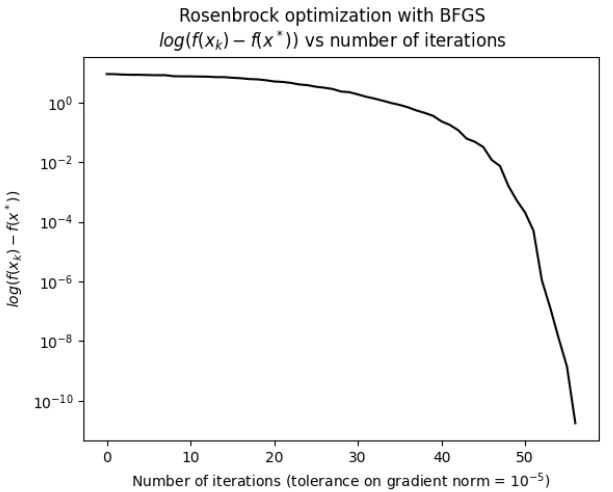
\includegraphics{rosenbrock_BFGS_plot.JPG}\\
The plot seems similar to the newton method rosenbrock convergence and is much better than simple gradient decent rate of convergence. 
\subsection{Neural Networks}
\stepcounter{subsubsection}
\stepcounter{subsubsection}
\stepcounter{subsubsection}
\subsubsection{Explicit Expression of the Neural Network Model}
\begin{itemize}
    \item Hidden layer 1:\\
$$x^1\in \mathbb{R}^{2}, W^1 \in \mathbb{R}^{2\times 4}, b^1\in \mathbb{R}^{4} $$
    \item Hidden layer 2:\\
$$x^2\in \mathbb{R}^{4}, W^2 \in \mathbb{R}^{4\times 3},  b^2\in \mathbb{R}^{3} $$
    \item Output layer:\\
$$x^3\in \mathbb{R}^{3}, W^3 \in \mathbb{R}^{3\times 1},  b^3\in \mathbb{R} $$
\end{itemize}
Now we calculate the layers' outputs:\\
$$x^1 = x$$
$$x^2 = \phi( W^{1^T} x^1 + b^1 )$$
$$x^3 = \phi( W^{2^T} \phi( W^{1^T} x^1 + b^1 ) + b^2)$$
$$F\left(x \vert \mathcal{W}\right) = \phi( W^{3^T} \phi( W^{2^T} \phi( W^{1^T} x^1 + b^1 ) + b^2) + b^3)$$
\stepcounter{subsubsection}
\stepcounter{subsubsection}
\subsubsection{Evaluating  the  Loss  Function’s  Derivative  with  Respect  to  Network’s Output of Single Training Example}
$$\frac{\partial L}{\partial F\left(x^i, \mathcal{W} \right)} = \frac{\partial }{\partial F\left(x^i, \mathcal{W} \right)}\{ \sum_{i=1}^{n} (F(x^i , \mathcal{W}) - y^i )^2\} = 2 (F(x^i , \mathcal{W}) - y^i)$$

\end{document}

